\documentclass{article}
\usepackage{amsmath}
\usepackage{amsfonts}
\usepackage{amssymb}
\usepackage[top=1.75cm,bottom=1.5cm,right=1.5cm,left=1.4cm]{geometry}
\setlength{\headheight}{22pt}
\usepackage{enumitem}
\usepackage{fancyhdr} % For customizing headers and footers
\usepackage{tikz}
\usepackage{pgfplots}
\pgfplotsset{compat=1.18}
\usepackage{caption} % for \captionof
\usepackage{subcaption}
\usetikzlibrary{angles,quotes,arrows.meta,calc}


%---------------- Header
\pagestyle{fancy}
\fancyhf{} % Clear default header and footer
\fancyhead[L]{{\footnotesize CUNEF Universidad \\ Bachelor in Philosophy, Politics and Economics}} 
\fancyhead[R]{{\footnotesize A. G. Azze \\ \date{2025}}} 
\setlength{\headsep}{1.2cm}
\fancypagestyle{plain}{
  \fancyhf{}
  \fancyhead[L]{{\footnotesize CUNEF Universidad \\ Bachelor in Philosophy, Politics and Economics}} 
  \fancyhead[R]{{\footnotesize A. G. Azze \\ \date{2025}}} 
}

%---------------- Title
\title{Math Essentials \\ Unit 5 - Trigonometric Functions}
\author{}
\date{}

\begin{document}
\maketitle

\section*{(Re)defining sine and cosine}

\subsection*{1) What does \(\sin(\theta)\) look like?}
\begin{enumerate}[leftmargin=0.7cm,label=(\roman*)]
  \item Plot the points \((\theta,\sin\theta)\) and observe the pattern.
  \item \textbf{Recall classical definition:} in a rectangle triangle,
    \[
    \sin(\theta)=\frac{\text{opposite}}{\text{hypotenuse}}.
    \]
  \item \textbf{Recall exact values:}  \(\sin(30^\circ)=\tfrac12\), \(\sin(45^\circ)=\tfrac{\sqrt2}{2}\), \(\sin(60^\circ)=\tfrac{\sqrt3}{2}\).
  \item \textbf{Acknowledge problem with classical definition:}
  What happens to \(0^\circ\) and \(90^\circ\)? What about angles outside the $[0^\circ, 90^\circ]$ interval? Why does the plot of $\sin$ extends to those angles if the classical definition breaks down? 
\end{enumerate}

\subsection*{2) A better definition: the unit circle}
Consider the \emph{unit circle} \(x^2+y^2=1\), centered at the origin. From the positive \(x\)-axis, rotate a radius of length \(1\) by an angle \(\theta\) to a point \(P=(x,y)\).
\[
\cos\theta=\frac{\text{adjacent}}{1}=x,\qquad \sin\theta=\frac{\text{opposite}}{1}=y
\quad\Rightarrow\quad P=(\cos\theta,\sin\theta).
\]
This works for all angles, including the previously problematic ones:
\[
\theta=0^\circ:\;P=(1,0)\Rightarrow \sin0^\circ=0,\ \cos0^\circ=1;\qquad
\theta=90^\circ:\;P=(0,1)\Rightarrow \sin90^\circ=1,\ \cos90^\circ=0.
\]

\subsection*{3) All quadrants: signs and symmetry}
As \(\theta\) increases, \(P(\cos\theta,\sin\theta)\) moves through the four quadrants.
\begin{itemize}[leftmargin=0.7cm]
  \item \textbf{Signs by quadrant \((\cos,\sin)\):} I:\((+,+)\), II:\((-,+)\), III:\((-,-)\), IV:\((+,-)\).
  \item \textbf{Reference angle \(\alpha\).} The acute angle to the $x$-axis; signs come from the quadrant.
\end{itemize}
\textbf{Examples.}
\[
\begin{aligned}
150^\circ \ (\text{QII, ref }30^\circ):&\quad \sin150^\circ=\tfrac12,\ \ \cos150^\circ=-\tfrac{\sqrt3}{2};\\
210^\circ \ (\text{QIII, ref }30^\circ):&\quad \sin210^\circ=-\tfrac12,\ \cos210^\circ=-\tfrac{\sqrt3}{2};\\
330^\circ \ (\text{QIV, ref }30^\circ):&\quad \sin330^\circ=-\tfrac12,\ \cos330^\circ=\tfrac{\sqrt3}{2}.
\end{aligned}
\]

\begin{figure}[ht]
\centering

% -------- Left: Unit circle --------
\begin{subfigure}{0.48\textwidth}
\centering
\begin{tikzpicture}[scale=2.8, >=Latex]
  % Angle
  \def\ang{35}
  \coordinate (O) at (0,0);
  \coordinate (X) at (1,0);
  \coordinate (P) at ({cos(\ang)},{sin(\ang)});
  \coordinate (Fx) at ({cos(\ang)},0);
  \coordinate (Fy) at (0,{sin(\ang)});

  % Axes
  \draw[->] (-1.2,0) -- (1.25,0) node[right] {$x$};
  \draw[->] (0,-1.2) -- (0,1.25) node[above] {$y$};

  % Unit circle
  \draw (O) circle (1);

  % Radius (hypotenuse = 1)
  \draw[thick] (O) -- (P) node[pos=0.55, above left=1pt] {\small $1$};

  % Triangle legs
  \draw[thick, blue] (O) -- (Fx) node[midway, below=2pt, blue] {\small $\cos\theta$};
  \draw[thick, red]  (Fx) -- (P) node[midway, right=2pt, red] {\small $\sin\theta$};

  % Angle arc
  \pic[draw,->,"$\theta$",angle eccentricity=1.25,angle radius=9mm] {angle = X--O--P};

  % Right angle marker
  \pic[draw,angle radius=4mm] {right angle = O--Fx--P};

  % Points
  \fill (P) circle (0.6pt)
        node[above right=2pt, font=\small] {$P=(\cos\theta,\sin\theta)$};
  \fill (1,0) circle (0.5pt) node[below right, font=\scriptsize] {$(1,0)$};
  \fill (0,1) circle (0.5pt) node[above left,  font=\scriptsize] {$(0,1)$};

  % Quadrant labels
  \node[font=\scriptsize] at (0.92,0.92) {QI};
  \node[font=\scriptsize] at (-0.92,0.92) {QII};
  \node[font=\scriptsize] at (-0.92,-0.92) {QIII};
  \node[font=\scriptsize] at (0.92,-0.92) {QIV};
\end{tikzpicture}
\caption{Unit circle: $P=(\cos\theta,\sin\theta)$.}
\end{subfigure}
\hfill
% -------- Right: sine & cosine --------
\begin{subfigure}{0.48\textwidth}
\centering
\begin{tikzpicture}
\begin{axis}[
  width=\linewidth, height=0.9\linewidth,
  axis lines=middle,
  xmin=0, xmax=360,
  ymin=-1.1, ymax=1.1,
  xtick={0,90,180,270,360},
  xticklabels={$0^\circ$,$90^\circ$,$180^\circ$,$270^\circ$,$360^\circ$},
  ytick={-1,-0.5,0,0.5,1},
  grid=both,
  grid style={line width=.1pt, draw=gray!30},
  major grid style={line width=.2pt, draw=gray!55},
  xlabel={$\,\theta$}, ylabel={},
  legend style={at={(0.5,1.05)}, anchor=south, draw=none, legend columns=-1}
]
  \addplot[domain=0:360, samples=500, smooth, very thick, red] {sin(x)};
  \addlegendentry{$\sin\theta$}
  \addplot[domain=0:360, samples=500, smooth, very thick, blue] {cos(x)};
  \addlegendentry{$\cos\theta$}
\end{axis}
\end{tikzpicture}
\caption{$\sin\theta$ (red) and $\cos\theta$ (blue), $0^\circ\!\le\!\theta\!\le\!360^\circ$.}
\end{subfigure}

\end{figure}


\subsection*{4) From circle to wave: the sine curve}
Plot the \(y\)-coordinate of \(P\) against \(\theta\in[0^\circ,360^\circ]\) to get the sine wave.
\[
\text{Amplitude }1,\quad \text{period }360^\circ,\quad
\sin\theta=0 \text{ at } \theta=0^\circ,180^\circ,360^\circ, \quad
\max=1 \text{ at } 90^\circ,\ \min=-1 \text{ at } 270^\circ.
\]

\subsection*{5) Angles: Degrees vs Radians}
\begin{minipage}{0.5\textwidth}
    \vspace{-5.4cm}
    \begin{itemize}[leftmargin = 0.3cm, label = $\bullet$, rightmargin = 0cm]
        \item \textbf{}\textbf{Why do we have degrees and radians?} 
        \begin{itemize}[leftmargin = 0.3cm, label = $\bullet$, rightmargin = 0cm]
            \item[] \textbf{Degrees are from the observer's perspective.} \\
            \noindent e.g., how many angles do you have to tilt your head up to see a planet?
            \item[] \textbf{Radians are from the mover's perspective.} \\
            \noindent e.g., what's the (relative) distance traveled by the planet?
        \end{itemize}
                            
        \item \textbf{Why radians are the standard in mathematics?} \\
        Taking the mover's perspective results in simpler notation
        
        \item \textbf{Why are there $\pmb{360^\circ}$?} \\
        Astronomers noticed that every day the stars were a bit (degree) off, and after about $360$ days they were back to their original position. That is due to the difference between a solar day ($24$ hours) and a sidereal day ($\approx$ $23$ hours and $56$ minutes)

        \item \textbf{Why radians are $\pmb{\pi}$-based?} \\
        The circumference of the unit-radius circle is $2\pi$.
    \end{itemize}    
\end{minipage}
\hspace{1.4cm}
\begin{minipage}{0.4\textwidth}
    
\includegraphics[width = \textwidth]{img/degree-radian.png}
    {\hspace{-0.1cm} 
\includegraphics[width = 0.9\textwidth, height = 8cm]{img/solar-sideral.png}}
\end{minipage}

\newpage
\section*{Exercises}

\begin{enumerate}[label=\textbf{\arabic*.}, leftmargin=*, itemsep=0.6em]
    \item Fill in:
    \begin{enumerate}[leftmargin=0.8cm]
        \item \(\sin270^\circ=\underline{\ \ \ \ }\), \ \(\cos270^\circ=\underline{\ \ \ \ }\).
        \item \(\sin120^\circ=\sin\underline{\ \ \ \ }\), \ \(\cos120^\circ=-\cos\underline{\ \ \ \ }\).
        \item The sign of $\sin290^\circ$ is $\underline{\qquad \qquad}$, and the sign of and \(\cos300^\circ\) is $\underline{\qquad\qquad}$.
    \end{enumerate}

    \item 
    Using only the unit-circle definition of \(\cos\theta\) and \(\sin\theta\), prove each of the following identities.
    \begin{enumerate}[leftmargin=0.8cm]
      \item \(\sin^2\theta+\cos^2\theta=1\).
      \item \(\sin(-\theta)=-\sin\theta\) and \(\cos(-\theta)=\cos\theta\).
      \item \(\sin(\tfrac{\pi}{2}-\theta)=\cos\theta\) and \(\cos(\tfrac{\pi}{2}-\theta)=\sin\theta\).
      \item \(\sin(\pi-\theta)=\sin\theta\) and \(\cos(\pi-\theta)=-\cos\theta\).
      \item \(\sin(\theta+\pi)=-\sin\theta\) and \(\cos(\theta+\pi)=-\cos\theta\).
      \item \(\sin(\theta+2\pi)=\sin\theta\) and \(\cos(\theta+2\pi)=\cos\theta\).
    \end{enumerate}    

    \item State the domain and codomain of the $\sin$ and $\cos$ functions.

    \item A child enters a carousel of unit radius that takes one minute to spin once around. The child enters at the point $(1, 0)$, that is, on the east position. Assume the carousel spins counter clockwise.
    \begin{enumerate}[leftmargin=0.8cm]
        \item What are the coordinates of the child after 45 seconds?
        \item What are the coordinates of the child after 90 seconds?
        \item What is the coordinates of the child after 125 seconds?
        \item When will the child have coordinates $(\sqrt{2}/2, -\sqrt{2}/2)$ if the ride lasts $6$ minutes? (There are multiple answers.)
    \end{enumerate}
    
    \item Solve for $x$: $4^{\sin^2(x)} + 4^{\cos^2(x)} = 5$.
    
    \item Consider a clock with an hour hand and a minute hand. What is the measure of the angle the minute hand traces in \(20\) minutes?
    
\end{enumerate}

\section*{Solutions}

\begin{enumerate}[label=\textbf{\arabic*.}, leftmargin=*, itemsep=0.6em]
  \item
  \begin{enumerate}[leftmargin=0.8cm]
    \item \(\sin270^\circ=-1\), \(\cos270^\circ=0\).
    \item \(\sin120^\circ=\sin 60^\circ\), \(\cos120^\circ=-\cos 60^\circ\).
    \item \(\sin290^\circ\) is \(\text{negative}\); \(\cos300^\circ\) is \(\text{positive}\).
  \end{enumerate}

  \item
  \begin{enumerate}[leftmargin=0.8cm]
    \item On the unit circle \(x^2+y^2=1\) with \(x=\cos\theta,\ y=\sin\theta\):
      \(\sin^2\theta+\cos^2\theta=y^2+x^2=1\).
    \item Reflecting angle \(\theta\) across the \(x\)-axis changes \(y\) to \(-y\) and keeps \(x\):
      \(\sin(-\theta)=-\sin\theta,\ \cos(-\theta)=\cos\theta\).
    \item Rotating by \(90^\circ\) swaps coordinates: \((x,y)\mapsto(y,x)\) with signs in QI:
      \(\sin(\tfrac{\pi}{2}-\theta)=\cos\theta,\ \cos(\tfrac{\pi}{2}-\theta)=\sin\theta\).
    \item Reflection across the \(y\)-axis: \((x,y)\mapsto(-x,y)\):
      \(\sin(\pi-\theta)=\sin\theta,\ \cos(\pi-\theta)=-\cos\theta\).
    \item Rotation by \(\pi\): \((x,y)\mapsto(-x,-y)\):
      \(\sin(\theta+\pi)=-\sin\theta,\ \cos(\theta+\pi)=-\cos\theta\).
    \item Full turn: \((x,y)\mapsto(x,y)\):
      \(\sin(\theta+2\pi)=\sin\theta,\ \cos(\theta+2\pi)=\cos\theta\).
  \end{enumerate}

  \item Domain: \(\mathbb{R}\) (all real angles). Codomain: \([-1,1]\) for both \(\sin\) and \(\cos\).

  \item Angular speed \(\omega=2\pi/60=\pi/30\ \mathrm{rad/s}\), position at time \(t\) (s): \((\cos\omega t,\ \sin\omega t)\).
  \begin{enumerate}[leftmargin=0.8cm]
    \item \(t=45\): \(\theta=\tfrac{\pi}{30}\cdot45=\tfrac{3\pi}{2}\Rightarrow(0,-1)\).
    \item \(t=90\): \(\theta=\tfrac{\pi}{30}\cdot90=3\pi\equiv\pi\Rightarrow(-1,0)\).
    \item \(t=125\): \(\theta=\tfrac{\pi}{30}\cdot125=\tfrac{25\pi}{6}\equiv\tfrac{\pi}{6}\Rightarrow\bigl(\tfrac{\sqrt3}{2},\tfrac12\bigr)\).
    \item Need \((\cos\theta,\sin\theta)=(\tfrac{\sqrt2}{2},-\tfrac{\sqrt2}{2})\Rightarrow\theta= \tfrac{7\pi}{4}+2k\pi\).
          Times \(t=\theta/\omega=30(7/4+2k)\) s \(=52.5+60k\) s.
          On a \(6\) min ride (\(0\le t\le360\)): \(t=52.5,\,112.5,\,172.5,\,232.5,\,292.5,\,352.5\) s.
  \end{enumerate}

  \item Let \(a=\sin^2 x\). Then \(\cos^2 x=1-a\) and
    \[
    4^{\sin^2 x}+4^{\cos^2 x}=4^{a}+4^{1-a}=5.
    \]
    Set \(t=4^{a}>0\). Then \(4^{1-a}=4\cdot 4^{-a}=4/t\), so
    \[
    t+\frac{4}{t}=5 \quad\Longrightarrow\quad t^2-5t+4=0
    \quad\Longrightarrow\quad t\in\{1,4\}.
    \]
    If \(t=1\), then \(4^{a}=1\Rightarrow a=0\Rightarrow \sin^2 x=0\Rightarrow x=k\pi\).
    If \(t=4\), then \(4^{a}=4\Rightarrow a=1\Rightarrow \sin^2 x=1\Rightarrow x=\frac{\pi}{2}+k\pi\).
    
    Hence the solutions are
    \[
    x=\tfrac{\pi}{2}k,\ \ k\in\mathbb{Z}
    \]

  \item Minute hand: \(360^\circ\) in \(60\) min \(\Rightarrow 6^\circ/\text{min}\).
        In \(20\) min: \(120^\circ=\frac{2\pi}{3}\ \text{rad}\).

\end{enumerate}


\end{document}
